\documentclass[12pt]{rapport}
\usetikzlibrary{%
  calc,%
  decorations.pathmorphing,%
  fadings,%
  shadings%
}
\usepackage{physics}
\usepackage{fixltx2e}
\usepackage{textcomp}
\course{34319: Programming Projects in IT and Communication Technology}

\title{Voix-er: VoIP/IM application}
\author{
  Martin Madsen (s124320)\\
  Christian Laustsen (s124324)
}
\date{28. Juni 2013}

\begin{document}
\maketitle

\section*{Introduction}
The program features a server and a client. It supports basic IM with
personal messaging and chat rooms that allow several users to interact
with each other in real time. Furthermore, the application also
implements VoIP (voice over IP), which allows the users to talk
directly to one another.\newline


The server-side part of the application is mainly written by Christian
(s124324), and the client-side of the application is mainly written by
Martin (s124320), although some sparring has been going on, as is
natural.


\section*{Requirements}
The following is a list of requirements that were specified for the
program when the project started. Some have been dumped or had failed
attempts of implementation.

\subsection*{Implemented}
\begin{itemize}
  \item A server that will allow multiple clients to connect
  \item A way to keep track of connected clients and their information
    (nicknames etc)
  \item Support for IM in the application
  \item A protocol for establishing a connection with the server and
    for the IM part of the application
  \item Chat rooms where several people can chat together at the same
    time
  \item A default channel where people are put when they connect
\end{itemize}

\subsection*{Not implemented}
\begin{itemize}
  \item Group VoIP chat
\end{itemize}


\section*{Design \& Implementation}
The server-side of the application is divided into several files which
each hold their own class. Each class is called the same as its file
(ie. channel.py holds the class Channel, and talk\_action.py holds the
class TalkAction).

\subsection*{main.py}
The main.py file is responsible for launching the two threads for the 
TCP and UDP server respectively. It also handles the gracefull shutdown 
of these two when the programme is aborted with Ctrl-C.

\subsection*{tcp\_server.py}
>>>>>>> Stashed changes
The TCPServer class is the main class of the server. It keeps track of
connected clients and when they are ready to be read from or written
to. It also provides an easy access to queue messages on the client
objects. The Server class is also responsible for PINGing the clients
periodically. The server class is the one the instantiates new Client
objects.

\subsubsection*{tcp\_client.py}
The TCPClient class takes care of the TCP connected clients (usually
IM, and also used to initiate the UDP client). It keeps track of when
it was pinged, its own User object, the message queue for the
socket/client etc. The TCPClient is also the one that instantiates new
Channel objects when needed (or reuses them if the channel already
exists).

\subsection*{udp\_server.py}
The UDPServer class takes care of the UDP connections, and sending them 
to the right "conversation" based on their session keys.

\subsection*{parser.py}
>>>>>>> Stashed changes
The Parser class handles the underlying protocol. It manages joins,
pings, messages, connections, disconnections etc. It interacts with
the Server and the Client/User object. Lastly, the Parser is also
responsible for instantiating new Talk objects in new threads when
necessary (and uses TalkAction objects to handle actions related to
the talk protocol).

\subsubsection*{channel.py}
The Channel class gathers information about the channel, and what
users are in it, along with giving quick methods for etc cleaning up a
channel. The channel object holds a static dictionary (hashmap) of all
the channel names pointing to their channel objects. This provides an
easy way to avoid channel name duplication.

\subsubsection*{user.py}
The User class holds the user data, and provides easy access to
leaving or joining a channel. The User class holds a static list of
all user nicknames (represented in strings), which allows the server
to quickly determine if the nickname is already is in use.

\subsubsection*{talk.py}
The Talk class takes care of the VoIP chat sessions, and manages the
UDP clients that are connected/linked to it. It has a session key, to
provide a quick way of referencing what Talk object (what
conversation) the client needs to enter. It waits for a TalkAction
object to perform some action (if it doesn't get one it 30 seconds, it
closes since the connection is seen as dead).

\subsection*{talk\_action.py}
The TalkAction class simply holds the instigator, action and the target 
of said the talk action, that is used in the Talk object.

\subsection*{talk\_data.py}
The TalkData class simply holds the the data of the UDP payload, and 
the address of the sender.

\subsection*{Client}
The client has the following architecture as seen on the UML
diagrams below. Each class is described in details in the sub-sections.
\begin{figure}[H]
  \begin{center}
    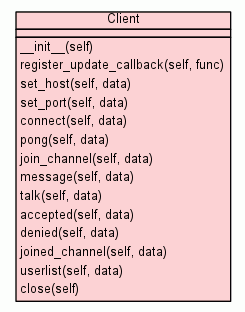
\includegraphics[scale=0.9]{../uml/uml_class_diagram_for_voix_cli}
    \caption{The structure of the Client class which is the main class,
      that operates on almost all the other classes.}
  \end{center}
\end{figure}
\begin{figure}[H]
  \begin{center}
    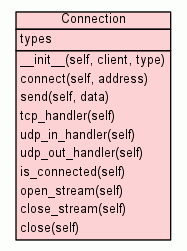
\includegraphics[scale=0.9]{../uml/uml_class_diagram_for_voix_con}
    \caption{The structure of the Connection class that handles TCP
      and UDP sockets.}
  \end{center}
\end{figure}
\begin{figure}[H]
  \begin{center}
    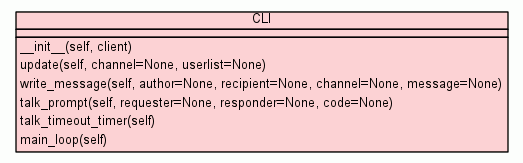
\includegraphics[scale=0.9]{../uml/uml_class_diagram_for_voix_int}
    \caption{The structure of the CLI class.}
  \end{center}
\end{figure}
\begin{figure}[H]
  \begin{center}
    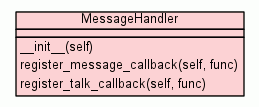
\includegraphics[scale=0.9]{../uml/uml_class_diagram_for_voix_mes}
    \caption{A message handler that lets interfaces register a
      callback to message and talk actions.}
  \end{center}
\end{figure}
\begin{figure}[H]
  \begin{center}
    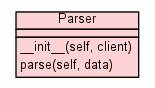
\includegraphics[scale=0.9]{../uml/uml_class_diagram_for_voix_par}
    \caption{The command parser that both translates stdin input and
      data received from the server.}
  \end{center}
\end{figure}
\subsubsection*{client.py}
All client operations are kept here and is the core part of the
application. The parser calls the methods defined here. This could be
connecting, setting hostname, join a channel etc.
\subsubsection*{connection.py}
TCP and UDP sockets are set up here to keep any connection-related
operations in one place. Threads are instantiated here to handle
incoming data from the server.
\subsubsection*{message\_handler.py}
This class is mainly a bridge between interfaces and the
core. Interfaces register callback functions that the core then
calls. The core does not have to know whether the interface is
graphically or something else.
\subsubsection*{parser.py}
Parser handles all the input from stdin and the server. Using regular
expressions all input is divided up into a list of the length $4$. The
first value is the command that is used to look up which function to
call. The remaining values are sent as arguments to this function.
\subsubsection*{cli.py}
The command line interface which is the only working interface. This
class holds the main program loop that reads from stdin. Commands may
be entered directly from the command line. For instance the server
host is set by writing ``HOST localhost'' and connecting is then
``CONNECT nickname fullname''. The client's version is automatically
parsed from the newest tag by the version control system, git.
\subsubsection*{gui.py}
The GUI class is to be defined here properly set up with wxWidgets. At
this moment it doesn't have much functionality. Therefore any
interaction with the client must happen using the CLI.

\section*{Protocol}
For the application, a custom protocol has been made. The following is
a list with an explanation of all the protocol commands/actions.

\subsection*{CONNECT}
\begin{verbatim}
From    - Client
Syntax  - CONNECT: <nickname> <realname> version number
Example - CONNECT: "John87" "John Wilson" 1.0.0
\end{verbatim}

\noindent The CONNECT action is sent when the client makes the initial
connection. Without this, the client cannot proceed further since all
commands will be seen as invalid if the user hasn't authenticated
himself with this.

\subsection*{ACCEPT}
\begin{verbatim}
From    - Server
Syntax  - ACCEPT: <hostname>
Example - ACCEPT: ip.google.com
\end{verbatim}

\noindent The ACCEPT action is sent to the client to acknowledge the
CONNECT.

\subsection*{NOTACCEPTED}
\begin{verbatim}
From    - Server
Syntax  - NOTACCEPTED: <message>
Example - NOTACCEPTED: Syntax error, please resend the CONNECT request
\end{verbatim}

\noindent The NOTACCEPTED action is sent when either there is a syntax
error in the CONNECT, or when the CONNECT hasn't been sent.

\subsection*{NICKNAMEINUSE}
\begin{verbatim}
From    - Server
Syntax  - NICKNAMEINUSE: <message>
Example - NICKNAMEINUSE: The nickname 'John83' is already taken
\end{verbatim}

\noindent The NICKNAMEINUSE action is sent when the nickname that the
user sent in with the CONNECT is already in use.

\subsection*{PING}
\begin{verbatim}
From    - Server
Syntax  - PING: <random number>
Example - PING: 42313812731
\end{verbatim}

\noindent The server keeps track of if clients are still connected by
sending them a PING periodically, and expecting a return PONG from
them with the same number as the PING had.

\subsection*{PONG}
\begin{verbatim}
From    - Client
Syntax  - PONG: <random number recieved from PING>
Example - PONG: 42313812731
\end{verbatim}

\noindent The client sends a PONG as a response to a PING to let the
server know that it is actually connected, and isn't a faulty
connection (or that it has a latency higher than a set amount of
seconds, which is 150 by default).

\subsection*{JOIN}
\begin{verbatim}
From    - Client
Syntax  - JOIN: <channel>
Example - JOIN: \#SuperAwesomeChannel
\end{verbatim}

\noindent Send a request to the server to join a channel.

\subsection*{JOINED}
\begin{verbatim}
From    - Server
Syntax  - JOINED: <channel>
Example - JOINED: \#SuperAwesomeChannel
\end{verbatim}

\noindent Respond to the client that it has successfully joined a channel.

\subsection*{USERLIST}
\begin{verbatim}
From    - Server
Syntax  - USERLIST <channel>: <comma separated list of users>
Example - USERLIST \#SuperAwesomeChannel: Will, John83, Mike
\end{verbatim}

\noindent This is send right after the JOINED action, and lists all
the users in the channel including the user itself (the client is
responsible for filtering this out).

\subsection*{USERJOIN}
\begin{verbatim}
From    - Server
Syntax  - USERJOIN <channel>: <nickname>
Example - USERJOIN \#SuperAwesomeChannel: Thomas12
\end{verbatim}

\noindent Notify the client that a user has joined a channel.

\subsection*{USERLEAVE}
\begin{verbatim}
From    - Server
Syntax  - USERLEAVE <channel>: <nickname>
Example - USERLEAVE \#SuperAwesomeChannel: Thomas12
\end{verbatim}

\noindent Notify the client that a user has left a channel.

\subsection*{MSG}
\begin{verbatim}
From    - Client
Syntax  - MSG <recipient>: <message>
Example - MSG \#SuperAwesomeChannel: Hey all! How's it going?
Example - MSG John83: Hey John! How's it going?
\end{verbatim}

\noindent The client can either send a message to a channel (where all
clients in that channel receives it), or directly to a user.

\subsection*{MSG}
\begin{verbatim}
From    - Server
Syntax  - MSG <sender> <recipient>: <message>
Example - MSG Thomas12 \#SuperAwesomeChannel: Hey all! How's it going?
Example - MSG Thomas12 John83: Hey John! How's it going?
\end{verbatim}

\noindent The server notifies either all the clients in a channel, or
just one client directly, that a message has been sent to them and
where the message stems from.

\subsection*{TALK (REQUEST)}
\begin{verbatim}
From    - Client
Syntax  - TALK <nickname>: REQUEST
Example - TALK John83: REQUEST
\end{verbatim}

\noindent Request a VoIP conversation with John83.

\subsection*{TALK (REQUEST)}
\begin{verbatim}
From    - Server
Syntax  - TALK <nickname> <session key>: REQUEST
Example - TALK John83 827742843590392: REQUEST
Example - TALK Mike 827742843590392: REQUEST
\end{verbatim}

\noindent The one that requested the conversation (let's say John83
did this) recieves this messages with the nickname being the one he
requested. He then needs to store the session key for later use in the
conversation.
\noindent The one that recieves the request (which will be Mike in
this case) will get the nickname of the requester in place of
nickname. The reciever will also need to store the session key, for
when he answers back.

\subsection*{TALK (ACCEPT/DENY)}
\begin{verbatim}
From    - Client
Syntax  - TALK <session key>: ACCEPT
Syntax  - TALK <session key>: DENY
Example - TALK 827742843590392: ACCEPT
Example - TALK 827742843590392: DENY
\end{verbatim}

\noindent To continue the example from before, the one that got the
request (Mike), will either accept or deny the request, and will send
the matching action to the server.

\subsection*{TALK (ACCEPTED/DENIED)}
\begin{verbatim}
From    - Client
Syntax  - TALK <session key>: ACCEPTED
Syntax  - TALK <session key>: DENIED
Example - TALK 827742843590392: ACCEPTED
Example - TALK 827742843590392: DENIED
\end{verbatim}

\noindent Again, continuing the example, since the one that got the
reqeust (Mike) has now answered with either a ACCEPT or DENY, the
requester (John83) will now get a response from the server stating
whether or not the request got accepted. If the conversation is
accepted, the VoIP conversation is started, if it's denied, the
process is stopped.

\subsection*{TALKSESSION}
\begin{verbatim}
From    - Client
Syntax  - TALKSESSION: <session key>
Example - TALKSESSION: 827742843590392
\end{verbatim}

\noindent This is sent by the UDP client after a talk request has been
accepted. It initiates the talk session/conversation.

\subsection*{SESSIONERROR}
\begin{verbatim}
From    - Server
Syntax  - SESSIONERROR: <message>
Example - SESSIONERROR: Invalid session key '827742843590392'
\end{verbatim}

\noindent If the TALKSESSION sends a wrong (nonexistant) or invalid
session key, the server responds with a SESSIONERROR.

\subsection*{DISCONNECT}
\begin{verbatim}
From    - Client
Syntax  - DISCONNECT
Example - DISCONNECT
\end{verbatim}

\noindent Signals to the server that the user is disconnecting, and
allows the server to quickly clean up after the user.


\section*{Testing}
The client has a variety of tests to assure valid data while
developing. The client is tested by itself with a dummy server. The
dummy server is to make sure data sent from the client reaches the
server it is connected to. This does mean, that not all scenarios are
testable and therefore communication between the client and the real
server may cause unexpected results. In this situation the scenarios
are only testable by black-box testing.

The client code is approximately covered $91\%$. This coverage is
distributed on modules as seen in the following scheme.

\begin{verbatim}
  Name                   Stmts   Miss  Cover   Missing
  ----------------------------------------------------
  voix                       0      0   100%
  voix.client              101      7    93%   109, 148, 206, 217-218, 221-222
  voix.connection           68      4    94%   103, 107-110
  voix.interface             0      0   100%
  voix.interface.cli        68      9    87%   38, 92, 104, 117-118, 126-129
  voix.interface.gui         6      3    50%   17-19
  voix.message_handler       8      0   100%
  voix.parser               14      0   100%
  ----------------------------------------------------
  TOTAL                    265     23    91%
  ----------------------------------------------------------------------
  Ran 16 tests in 6.187s

  OK
\end{verbatim}

The test methods' names should explain the goal that is wished to
assert for. And the runtime of
{\fontfamily{ptm}\selectfont\texttildelow}$6$ seconds is caused by
delays to overcome threaded operations. This coverage may not be
up-to-date with the final code (mind changes to the TALK related
code).\newline

For the server, a fake client is made to overcome the same situation
as on the client. The test runs two fake clients in threads, and each have 
different tasks, and are made to simulate a response/interaction of two
clients on the server. They test both the TCP and the UDP part of the 
server, by initiating a call, and simply inputting plain text over the 
UDP protocol.

\section*{Possible features \& expansions}
Here's a list of additional brainstormed features and things that
should be done.
\begin{itemize}
\item Major code cleanup (mainly on the client) and possible
  rewrites of parts of the code that would simplify certain complex
  tasks.
\item Implement group VoIP chat
  % TODO: more features??
\end{itemize}


\newpage
\section*{Conclusion}
Unfortunately, we didn't quite reach the goals we set off with at the 
start of the project. Especially the group VoIP was one of our goals.

On the other hand, we've gotten some experience playing with TCP and UDP
sockets, and the programmatical restrictions and differences of using them,
in an actual program. 



\newpage
\section*{User guide}
The server is simply started by running $python main.py$ file in the 
root directory of the server (the server is called voixer). If less 
detailed output/logging is needed, it can easily be altered in the 
main.py file, along with the port to listen to (if the address is 
already in use).


\end{document}